\documentclass[a4paper,prd,twocolumn,nofootinbib,superscriptaddress,floatfix]{revtex4}
%\documentclass[prd,twocolumn,nofootinbib,showpacs]{revtex4-1}

%\usepackage{amsmath,amssymb}
\usepackage{cancel}
\usepackage{graphicx}
\usepackage{epsfig}
\usepackage{physics}
\usepackage{amsmath,amsfonts,amssymb}
\usepackage{color,soul}
\newcommand{\myexp}{e^}
\usepackage{float}
\usepackage{graphicx}
\graphicspath{ {Images/} }
\usepackage[utf8]{inputenc}
\usepackage{hyperref}
\usepackage[compatibility=false]{caption}
\usepackage{subcaption}
\usepackage{eurosym}
\usepackage{siunitx}
\renewcommand*{\figureautorefname}{FIG.}

\begin{document}

\title{Sensitivity Analysis on Least-Squares American Options Pricing}

\author{Miguel Ângelo Maia Ribeiro}

\affiliation{Departamento de F\'{\i}sica, Instituto Superior T\'ecnico, Universidade de Lisboa, Lisboa, Portugal}
%\begin{document}



\maketitle
\section{Introduction}
The stock market has suffered a complete paradigm shift in the past decades. Recent developments in computer science and mathematical finance have greatly enhanced our abilities to predict and take advantage of stock price changes. It shouldn't come as much of a surprise that there has been an ever growing desire from investors to take advantage of these new developments to increase potential profits.

With the colossal sums handled daily in the stock market, even a small improvement on the predictive abilities of a given forecasting algorithm can lead to significant increases in profits for investors. In such a highly competitive subject, it should be clear that a great amount of resources should be devoted to the research and development of these algorithms. An investor that does not follow this strategy is bound to lose major profits when compared with his better prepared counterparts.




Due to the developments in stock price forecasting, our knowledge of derivatives has also greatly increased. A derivative is simply a contract whose value depends on other simpler financial instruments, like stocks or interest rates. Derivatives can virtually take any form desirable, so long as there are two parties interested in taking a part in it. In this work we will focus on the most common type of derivatives - options.

The derivatives market has become increasingly important in recent times. In fact, as of June 2017, derivatives are responsible for over $\$542$ trillion worth of trades, in the Over-the-Counter (OTC) market alone, as can be seen on \autoref{fig:OTC} (the OTC market refers to all deals signed outside of derivatives exchanges). Though the market size peaked in 2013 with over $\$710$ trillion, it seems to have shrinked in the last decade, which might be attributed to the global financial crisis of 2007.

\begin{figure}[H]
    \centering
      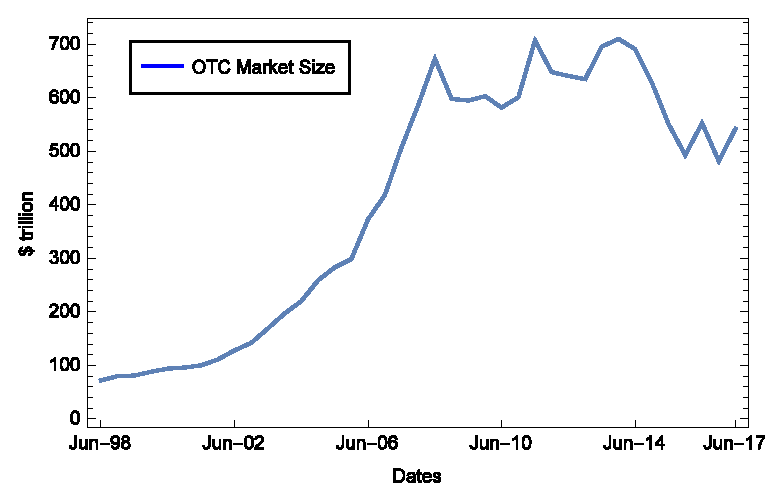
\includegraphics[width=.9\columnwidth,trim={2pt 17pt 0 0},clip]{OTC.eps}
      \caption{Size of OTC derivatives market.\newline \footnotesize{\textbf{Source:} stats.bis.org/statx/srs/table/d5.1 (on 16/11/2017)}}\label{fig:OTC}
    \end{figure}

\subsection{Call and Put Options}
Among the many types of derivatives, the most commonly traded are options, of which there are two main types - calls and puts.

In simple terms, a \textit{call option} grants the investor the right to buy the underlying asset (e.g. stock) for a fixed price, known as the \textit{strike price}, by a certain date, known as the \textit{expiration date}.\\
On the other hand, a \textit{put option} grants the investor the right to sell the underlying asset for the strike price, by the expiration date.\\
If at the time of exercise, the stock price is above (resp. below) the strike price, the owner of a call (resp. put) option should exercise his right to buy (resp. sell) the stocks, earning the difference between the stock price and the strike price. The payoff function of these two types of derivatives can then simply be deduced as
\begin{equation}\label{callput}
\begin{split}
&\text{Payoff}_\text{call}(t)=(S(t)-K)^+,\\
&\text{Payoff}_\text{put}(t)=(K-S(t))^+;
\end{split}
\end{equation}
\noindent where $K$ is the strike price and $S(t)$ is the stock price at the time of exercise, $t$.

\begin{figure}[H]
    \centering
      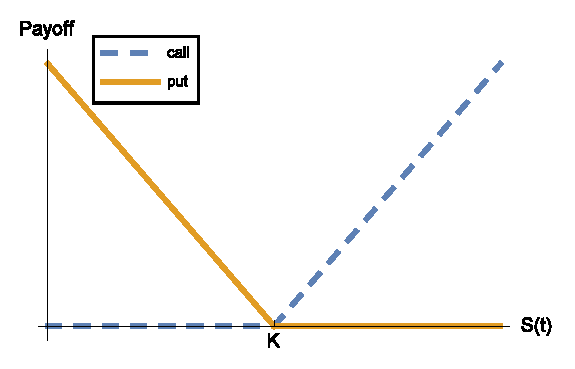
\includegraphics[width=.8\columnwidth]{Payoff.eps}
      \caption{Payoff functions of \textit{call} and \textit{put options}.}\label{fig:Payoff}
    \end{figure}

It's important to note that an option gives the holder the right to buy/sell the underlying asset but he is not obliged to do so. If exercising the option would lead to losses, the investor can simply let the option expire.



Options have several advantages that make them especially appealing to investors.
To hedgers (i.e. investors that want to limit their exposure to risk), options provide safety by fixing the future price of a stock. If a hedger is afraid of a stock price crash in the future in one of the stocks he holds, by buying put options he ensures that his losses are contained because he can always sell the stocks he owns for the fixed strike price, even if the price crashes.
To speculators (i.e. investors that want to take advantage of the uncertainty of future stock prices by betting on their outcome), options grant access to much larger profits when the market forecast proves true, with much smaller initial investments.


Because of all their advantages, unlike some other types of derivatives options have a cost. Finding the ideal price for an option is quite difficult, however. This pricing problem is a fundamental concern to investors, because under or overpricing an option could have severe consequences and lead to major losses.
The price of an option and what influences it will be the main focus of this work.




\subsection{European and American Options}
Both call and put options can be further separated into several categories. Among these, European and American options are by far the most commonly traded.
The holder of an \textit{European option} can only exert his right to buy/sell (call/put) the underlying assets, also known as \textit{exercising}, at the specified expiration date.
On the other hand, an \textit{American option} enables its owner to exercise it at any time up to its expiration date.



Due to their high importance, options have been studied in detail in the past.
Possibly the most important result in this field came from Robert Merton and Myron Scholes who earned the 1997 Nobel prize in Economics for developing a mathematical model to price European options - the famous Black-Scholes formula - still used nowadays, though with some modifications. Their result states that an European call or put option's price follows the partial differential equation (PDE)

\begin{equation}
\pdv{V}{t}+\frac{1}{2}\sigma^2S^2\pdv{V^2}{S^2}+rS\pdv{V}{S}-rV=0,
\end{equation}

\noindent where $V$ is the price of the option, $S$ is the price of the underlying stock, $r$ is the risk-free interest rate and $sigma$ is the stock price volatility.
This model assumes furthermore that stock prices follow a Geometric Brownian Motion (GBM), which can be defined as

\begin{equation}
dS(t)=rSdt+\sigma SdW(t),
\end{equation}
\noindent with W(t) defining a Brownian motion.

Pricing American options, however, poses a much greater challenge. Because they can be exercised at any time, the underlying assets must be closely monitored so as to attempt optimal stopping.
Furthermore, unlike European options, no analytic pricing model currently exists for this type of derivatives. Several numerical models have been proposed in the past in an attempt to price these options. Among these, Longstaff and Schwartz developed one of the most popular, based on Monte Carlo simulation with least squares regression to calculate the option price. Their results will be heavily used in this work.

Despite their complexity, American options are nonetheless very much used by investors. In fact, most of the options currently traded in exchanges are American. Thus, it is absolutely critical to understand which variables influence this type of derivatives and by what amount. With this knowledge, one can better prepare oneself to market changes and even mitigate potential risks.

\subsection{Sensitivity Analysis}
Many factors influence the final price of an option.
Some factors are absolutely defined, such as the option strike price or the expiration date, while others have an associated uncertainty, like the stock price volatility or the interest rate.

To fully understand how models with uncertain inputs work, a sensitivity analysis is required. In short, sensitivity analysis studies which factors have a greater effect on the final model output.
There are many types of sensitivity analysis that go from simple scatter plots to more complex variogram-based methods. One particularly useful type of analysis is the variance-based sensitivity analysis.

Initially created by Ilya Sobol in 1990 and later further developed by several people, among which the work by Andrea Saltelli is paramount, variance-based sensitivity analysis enables the knowledge of by how much the final model output's variance would decrease if we could completely nullify the uncertainty of a given input.
In option pricing this is particularly useful. If an investor knows where the greatest source of uncertainty of the option price comes from, he can invest greater sums in the mitigation of that uncertainty.

Due to its usefulness, this particular type of sensitivity analysis and its application to option pricing will be the main focus of this work.



\section{Objectives}
The main objective of this thesis is to perform a sensitivity analysis on the price of American options.

We will begin by replicating the model developed by Longstaff and Schwartz to price American options. Their method is based upon a Monte Carlo generation of stock price paths with a set of market variables such as stock price volatility and interest rate (using the Black-Scholes stochastic differential equation). To these results, a least squares regression is then applied iteratively to generate an optimal stopping decision matrix with all the stock price paths generated.

Having replicated this algorithm, we shall then apply a variation-based sensitivity analysis, as developed by Sobol and Saltelli. This analysis outputs a weight for each of the variables used proportional to their influence in the variance of the final option price.
Thus, if a variable has a large weight, its variance has a large impact in the variance of the option price.

Some other aspects of this sensitivity analysis will also be considered, such as how each variable's weight changes with time.

As a next step, we shall modify the Longstaff-Schwartz method to more closely resemble real-world stocks.
We might, for example, implement the GARCH(1,1) model for the stock price volatility to account for daily changes on its value. We could also try to implement interest rate models for the same reason.
Some more recent studies of the Longstaff-Schwartz algorithm suggest that a more effective method to price American options would consist of replacing the least squares regression by some other numerical method, related to optimal stopping.
A further study of which models better suit our needs is still necessary, however, and perfecting the initial algorithm will also be a major section of this thesis.


Finally, we will try to apply our model to real-world stock prices, publicly available, and perform this sensitivity analysis using this data.



\section{State of the art}


\section{Commented Bibliography}
\subsection{Miscellaneous Topics}
John Hull's book is a great source for most option related information. In this book, Hull explains most option market mechanics and some recent results in this field. In what concerns the present work, the most important topic explored in the book is related to the GARCH(1,1) model.
\begin{itemize}
\item Hull, J. (2012). \textit{Options, futures, and other derivatives}. Boston: Prentice Hall.
\end{itemize}

\subsection{American Option Pricing}
Longstaff and Schwartz's paper on the pricing of American options will be heavily used throughout this work. Most results will be based on some variation of their algorithm. Their paper is not only important for the results it presents but also for the examples it provides that enable a clear and deep understanding of the algorithm.
\begin{itemize}
\item Longstaff, F. A., \& Schwartz, E. S. (2001, January 1). Valuing American Options by Simulation: A Simple Least-Squares Approach. \textit{The Review of Financial Studies, 14}(1), 113-147.
\end{itemize}

This book presents some useful simulations of many option based results. Though Chloe presents no new results in the option pricing field, some of the simulations developed in this thesis may be based, up to some extent, in the ones presented in Chloe's book.
\begin{itemize}
\item Choe, G. H. (2016). \textit{Stochastic Analysis for Finance with Simulations}. Universitext. Springer International Publishing. 
\end{itemize}

\subsection{Sensitivity Analysis}
Sobol


Saltelli

\section{Timetable}

\iffalse
\section{Thesis Supervisors}
\begin{itemize}
  \item Cláudia Nunes Philippart, \ \ cnunes@math.tecnico.ulisboa.pt
  \item Rui Manuel Agostinho Dilão, \ \ ruidilao@tecnico.ulisboa.pt
  \item Claude Yves Cochet, \ \ claude.cochet@bnpparibas.com
\end{itemize}
\fi

\end{document}

\iffalse
Among these, the most commonly traded are call and put options. In short, a call (resp. put) option gives an investor the right to buy (resp. sell) a particular stock for a fixed price (called the strike price) at some point in the future. If the stock price increases above (resp. decreases below) the fixed price, the investor can simply buy the said stock in the stock market for the lower fixed (resp. current) price, and sell it immediately after for the higher current (resp. fixed) price, earning the difference. If, otherwise, the stock price goes down (resp. up), then the option is worthless and the investor loses his investment.\\
The payoff functions can be easily deduced as
\begin{equation}\label{callput}
\begin{split}

\end{split}
\end{equation}
\noindent where $K$ is the strike price and $S(t)$ is the stock price at the time of exercise, $t$.\fi
\iffalse
In short, options magnify consequences: a good forecast turns into a large profit whereas a bad prediction results in a loss of investment.
\fi
\iffalse
For one, they limit the exposure to risk, e.g. if the price of a given stock were to crash, stock holders would lose a serious amount of funds whereas the owner of a call option would only lose his smaller original investment. On the other hand, options can also lead to greater profits e.g. using the same example of the stock price crash, the owner of a put option could buy this option for the lower current price (after the crash) and sell it for the higher price, fixed at the time of acquisition, before the crash happened.

This type of derivatives also comes with its own caveats. The main disadvantage is the fact that options always deal with stock prices in the future, i.e one can never precisely anticipate how much will be earned, if anything at all. Thus, it's clear that accurately modeling the stock price is paramount when dealing with options.
\fi
\iffalse
Call and put options are also divided into different types. The two most commonly used are European and American options. An European option can only be exercised - buying/selling the stocks for the fixed stock price with a call/put option - at a fixed date in the future, whereas an American option can be exercised anytime up until that fixed date. The payoffs of each of these types of options is simply
\begin{equation}
\begin{split}
&\text{Payoff}_\text{European}=\text{Payoff}_\text{call/put}(T);\\
&\text{Payoff}_\text{American}=\text{Payoff}_\text{call/put}(t), \ \ \ \forall 0<t<T,
\end{split}
\end{equation}

\noindent where $\text{Payoff}_\text{call/put}(t)$ corresponds to the payoffs from equations \ref{callput} and $T$ corresponds the fixed exercise date of European options.
\fi
\iffalse
When dealing with problems with no analytic solutions, such as the case of American options pricing, it becomes impossible to precisely predict how the model inputs directly affect the final output.

When dealing with inputs with an associated uncertainty, one must use sensitivity analysis to find how the model parameters influence the final result.

A sensitivity analysis simply outputs

Many factors have a weight in the final price of an option.
Because there is no analytic solution to price American options, we depend solely on numerical models to achieve this task.
\fi
\iffalse
First we will begin by simulating a large number of stocks, using the simple Black-Scholes formula to generate each path. The main point behind this method is to apply the Monte Carlo approach to the stock price which will be used later in the option pricing.
After generating all the paths, we shall attempt to replicate the method developed by Longstaff and Schwartz for pricing American options, using the results from the previous simulation.
Next, we will modify the initial simulations using more complex models that better replicate real-world stocks, such as varying volatility, varying interest rate. We shall further study which other factors influence the final price of an option.
We shall then apply a sensitivity analysis on the option price, using the model developed by Sobol and Saltelli.
\fi
\iffalse

\noindent Derivatives have become increasingly important in recent decades, with the sums currently handled in these markets amounting to several trillion dollars.\\
For this reason, it is of the utmost importance to be able to accurately predict the payoff of such contracts to correctly price them.\\
In this thesis we will study particularly the pricing of American options. These contracts are especially difficult to price due to the high uncertainty associated with optimal stopping.\\
Several methods have been suggested to achieve this goal, such as finite difference, but we shall use the procedure proposed by Longstaff et al., using Monte Carlo simulation and least-squares regression.\\
We will mainly focus on the sensitivity analysis of this pricing process, namely how the parameters’ volatility affects the final calculated price.\\
This analysis is particularly important due to the sometimes-large uncertainty associated with the parameters used. For this reason, we find that the least-squares approach is ideal under such conditions, since we expect it to be less sensitive to volatility than other methods.
\fi